\chapter{\huge Integrazione Numerica}

\textit{In analisi numerica, l'integrazione numerica consiste in una serie di metodi che stimano il valore di un integrale definito, senza dover calcolare la primitiva della funzione integranda. In questa sezione si illustrano alcuni dei principali metodi deterministici e non.}

\section{Newton-Cotes}
Le regole di quadratura di Newton-Cotes sono formule che consistono nel valutare l'integrando in punti equispaziati dell'intervallo di integrazione.

Si assume che il valore di una funzione $f:[a,b]\in\mathbb{R}\rightarrow\mathbb{R}$ sia noto nei punti $x_i$, per $i=0,...,n$ tali che $$x_i=a+\left(\frac{b-a}{n}\right)i$$
La formula di Newton-Cotes di grado $n$ si ottiene interpolando $f$ nei punti $x_i$ con i polinomi della base di Lagrange, e integrando la polinomiale risultante, $L(x)$, nell'intervallo $[a,b]$.
$$ \int_a^b f(x) \,dx \approx \int_a^b L(x)\,dx = \int_a^b \bigl( \sum_{i=0}^n f(x_i)\, \ell_i(x) \bigr) \, dx = \sum_{i=0}^n f(x_i) \underbrace{\int_a^b \ell_i(x)\, dx}_{w_i} $$
dove gli $\ell_i(x)$ sono i polinomi di Lagrange così definiti
$$\ell_i(x):= \prod_{\begin{smallmatrix}0\le j\le n\\ j\neq i\end{smallmatrix}} \frac{x-x_j}{x_i-x_j}$$$$\ell_i(x_j)=\delta_{ij}$$
La formula di Newton-Cotes assume così la semplice forma di media dei valori $f(x_i)$ pesati sui coefficienti $w_i$ (indipendenti da $f$)
$$\int_a^b f(x) \,dx \approx \sum_{i=0}^n w_i\, f(x_i)$$
Si domostra che l'errore sulla stima di $f$ dato dall'interpolazione polinomiale è
$$E(x)=\frac{1}{(n+1)!}f^{(n+1)}(\xi(x))\prod_{i=0}^n(x-x_i)$$
per un certo $\xi\in[a,b]$ dipendente da $x$. Non avendo tuttavia alcuna informazione su come individuare il punto $\xi$ in genere si effettua solo una stima del limite superiore sull'errore $E(x)$ per $\xi$ tale che $f(\xi) = \underset{x\in[a,b]}{\max}f(x)$.

Al primo ordine dell'approssimazione Newton-Cotes la formula si riduce al cosidetto metodo dei ``trapezi'':
$$\int_a^b f(x) \,dx=\frac{b-a}{2}\left[ f(a)+f(b)\right] + \underbrace{\frac{1}{2}\int_a^b f''(\xi(x))(x-a)(x-b)}_{E_1}$$
mentre al secondo ordine non è altro che la regola di Simpson:
$$\int_a^b f(x) \,dx=\frac{b-a}{3}\left[f(a)+4f(\frac{a+b}{2})+f(b)\right] + \underbrace{\frac{1}{6}\int_a^b f'''(\xi(x))(x-a)(x-\frac{a+b}{2})(x-b)}_{E_2}$$

\section{Quadrature Gaussiane}
La regola di quadratura Gaussiana a $n$-punti è un metodo di integrazione numerica costruito in modo tale da fornire un risultato esatto per polinomi di grado inferiore a $2n$, attraverso una scelta appropriata di punti $x_i$ e pesi $w_i$, per $i=0,...,n$. Sul dominio di integrazione convenzionale $[-1,1]$ la regola è così formulata
$$\int_{-1}^1 f(x)\,dx \approx \sum_{i=1}^n w_i f(x_i)$$


\section{Monte Carlo}

\section{Esempi}
\begin{figure}[h]
\centering
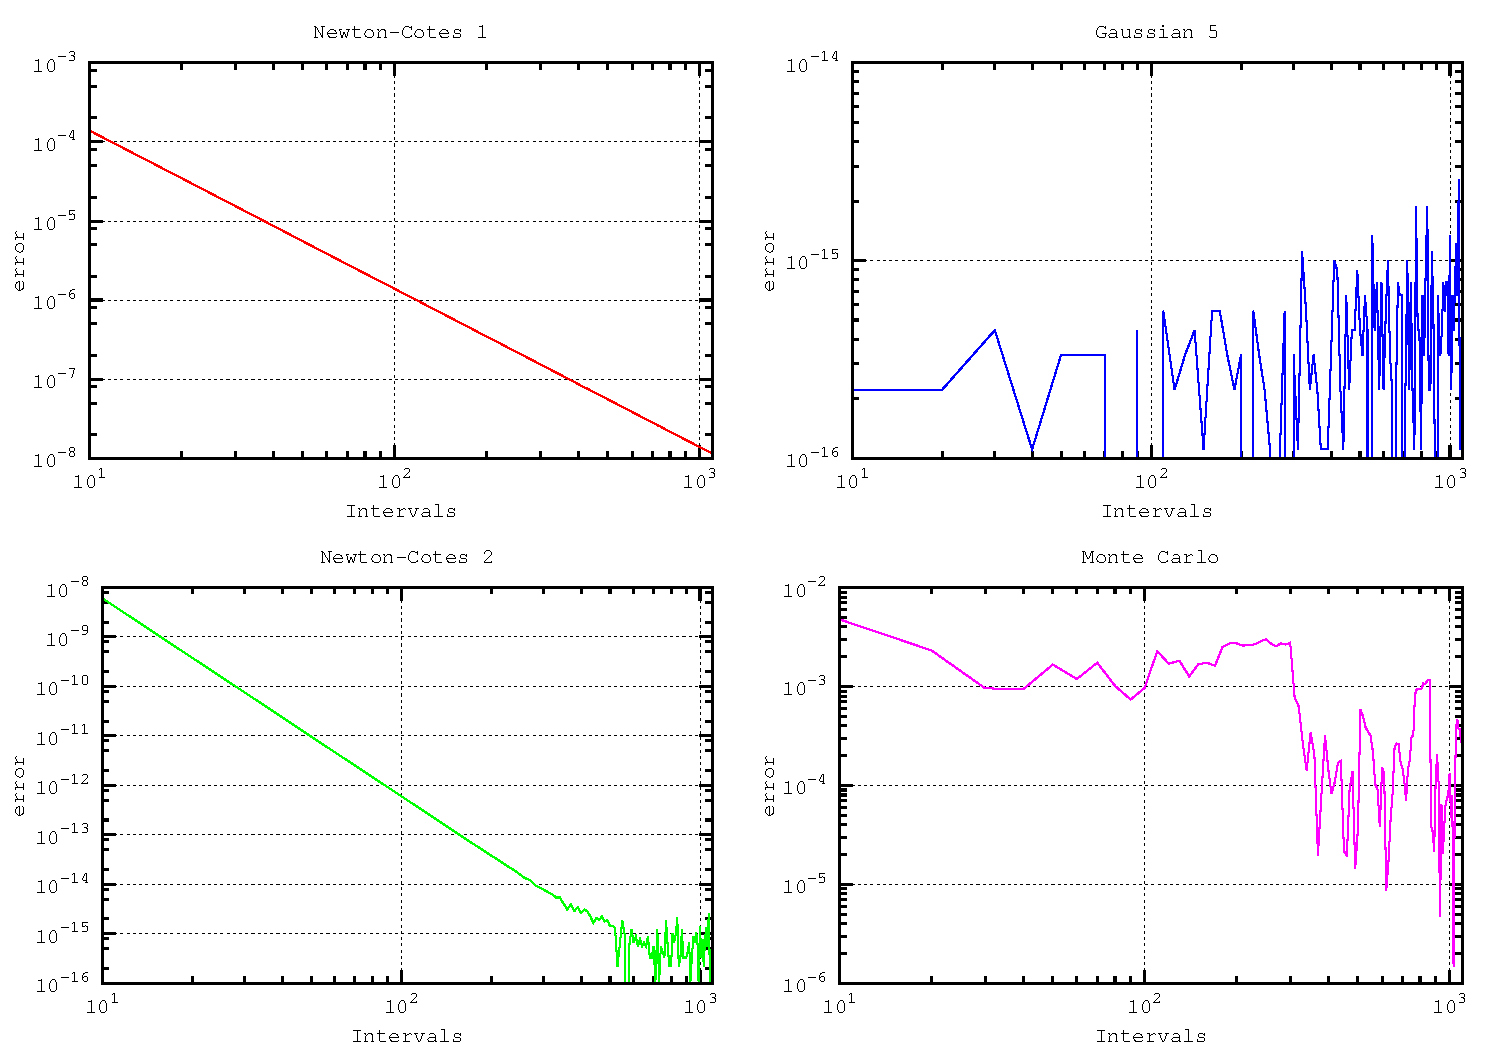
\includegraphics[width=\textwidth]{integral}
\caption{Errore calcolato}
\label{fig:integral}
\end{figure}

